\section{Theoretische Grundlagen}

In diesem Kapitel werden die grundlegenden Begriffe und Konzepte erläutert, welche wichtig für das Verständnis der Arbeit sind. Es wird zunächst der DevOps-Ansatz und das Architekturmuster der Microservices beschrieben. Im Anschluss werden die Grundlagen von Docker sowie Kubernetes erklärt.

\subsection{DevOps}

Alle der in diesem Kapitel beschriebenen Architekturmuster, Methoden und Werkzeuge lassen sich dem DevOps-Ansatz zuordnen. Um den Gesamtkontext zu verstehen, ist es deshalb sehr wichtig zu wissen, was DevOps bedeutet und warum es so populär ist. Wie das Kofferwort \glqq DevOps\grqq{} bereits andeutet, beschreibt es einen Ansatz für eine effektivere und stärkere Zusammenarbeit zwischen Softwareentwicklung (Development) und IT-Betrieb (Operations). Für DevOps gibt es keine einheitliche Definition. Es ist ein Überbegriff für Denkweisen, Kultur, Methoden, Technologien und Werkzeuge. Der Kundennutzen wird dabei immer in den Mittelpunkt gestellt \parencite[vgl.][S. 1]{halstenbergDevOps2020}. Das Ziel ist es die Softwarequalität zu verbessern sowie die Geschwindigkeit der Entwicklung und Bereitstellung zu erhöhen \parencite[vgl.][S. 6]{arundelCloud2019}. Um diese Ziele zu erreichen, werden etablierte Methoden und Werkzeuge eingesetzt. Die einzelnen Phasen der Entwicklung und des Betriebes bilden gemeinsam einen Prozess, der von jedem Programminkrement durchlaufen wird \parencite[vgl.][S. 63]{trempArchitekturen2021}.

\begin{figure}[H] 
    \centering
    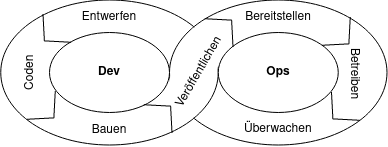
\includegraphics[width=0.75\textwidth]{figures/DevOpsKreislauf.png}
    \caption{Kreislauf und Schritte von DevOps \parencite[vgl.][S. 63]{trempArchitekturen2021}}
\end{figure}

Durch eine Automatisierung, \ac{CI} und \ac{CD} kann beispielsweise die Time-to-Market reduziert werden. Diese Kennzahl gibt an, wie lange es dauert eine Änderung zum Kunden, also auf die Produktionsumgebung, zu bringen \parencite[vgl.][S. 7]{halstenbergDevOps2020}. Auch Microservice-Architekturen und Werkzeuge wie Docker und Kubernetes können dabei unterstützen.

DevOps wird immer wichtiger, da durch das Aufkommen von Cloud Computing die Entwicklung und der Betrieb von Anwendungen schwieriger zu trennen ist. DevOps in ein Unternehmen einzuführen ist ein langwieriger Prozess. Neben der Einführung der neuen Technologien ist vor allem die Transformation der Unternehmenskultur besonders mühevoll. In großen Unternehmen zeigt sich das viele Prozesse schwerfällig geworden sind und nicht mehr dem eigentlichen Kundennutzen dienen. DevOps soll dieses Problem lösen und Unternehmen wieder anpassungsfähiger machen, ohne geordnete Strukturen zu verlieren.

\begin{figure}[H] 
    \centering
    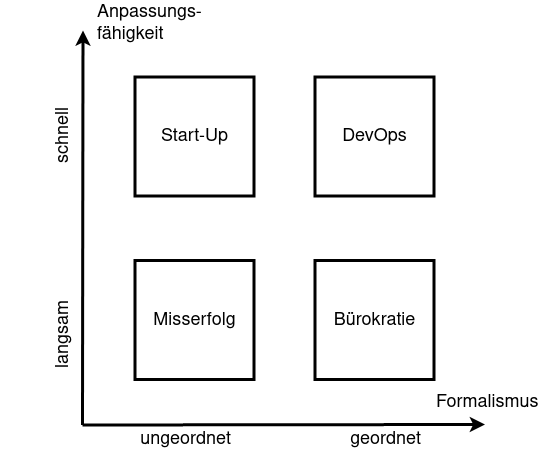
\includegraphics[width=0.7\textwidth]{figures/DevOpsKategroisierung.png}
    \caption{Kategorisierung von Unternehmen nach Anpassungsfähigkeit und Formalismus \parencite[vgl.][S. 11]{halstenbergDevOps2020}}
\end{figure}

\subsection{Microservices}
Im Mittelpunkt dieser Arbeit stehen Microservices. Bei Microservices handelt es sich um ein Architekturmuster zur Modularisierung von Software \parencite[vgl.][S. 15]{newmanMicroservices2015}. Eine einheitliche Definition für Microservices gib es nicht \parencite[vgl.][S. 2]{wolffMicroservices2018}. Bei der Beschreibung von Microservices werden Prinzipien und Merkmale einer standardisierten Definition vorgezogen. Im Folgenden werden die wichtigsten Merkmale kurz erläutert.

\subsubsection{Merkmale}
Microservices sind das Gegenteil von klassischen monolithischen Softwarearchitekturen. Ein Monolith ist eine einzelne, zusammenhängende und untrennbare Einheit. Die Erweiterbarkeit und Wartbarkeit von Monolithen ist häufig komplex, da die Codebasis umfangreich ist und mit der Zeit immer stärker wächst. Die Arbeit von mehreren Entwicklerteams ist ineffizient, da ein hoher Abstimmungsbedarf nötig ist. Des Weiteren ist die Skalierbarkeit des schwergewichtigen Monolithen sehr beschränkt. Durch Modularisierung des Monolithen lassen sich diese Probleme abschwächen, können jedoch nicht vollständig behoben werden.

\begin{figure}[H] 
    \centering
    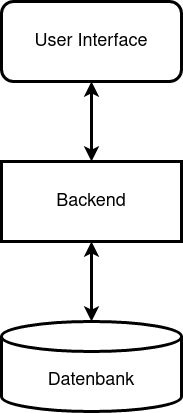
\includegraphics[width=0.2\textwidth]{figures/AufbauMonolith.png}
    \caption{Beispielhafter Aufbau einer monolithischen Architektur}
\end{figure}

Genau hier setzten Microservices an. Obwohl der Begriff Microservices noch realtiv jung ist, sind die dahinterstehenden Konzepte bereits deutlich älter \parencite[vgl.][S. 15]{newmanMicroservices2015}. Zur Verständlichkeit und leichteren Weiterentwicklung werden große Systeme schon lange in kleine Module unterteilt. Die Besonderheit von Microservices liegt darin, dass die Module einzelne Programme sind. Das Architekturmuster der Microservices zählt zu den verteilten Systemen. Die einzelnen Microservices laufen zumeist auf vielen unterschiedlichen Rechnern und kommunizieren über das Netzwerk.

\begin{figure}[H] 
    \centering
    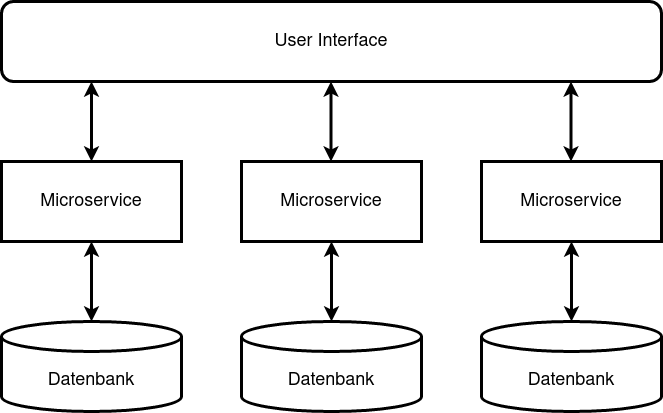
\includegraphics[width=0.71\textwidth]{figures/AufbauMicroservices.png}
    \caption{Beispielhafter Aufbau einer Microservice-Architektur}
\end{figure}

Ein einzelner Microservice soll eine Aufgabe bestmöglich erledigen. Dieser Ansatz ist angelehnt an die Philosophie von \acs{UNIX}: \glqq Mache nur eine Sache und mache sie gut\grqq{} \parencite[vgl.][]{salusQuarter1994}. Jeder Microservice bildet so eine klar definierte Funktion des Gesamtsystems ab \parencite[vgl.][S. 64]{trempArchitekturen2021}. Die Microservices müssen dabei eigenständig sein, sodass sie unabhängig voneinander verändert und bereitgestellt werden können. Die Kommunikation zwischen den Microservices erfolgt über das Netzwerk mittels sprachunabhängiger Schnittstellen, sogenannte \acp{API}. Um die Microservices unabhängig voneinander skalieren zu können, müssen sie zudem zustandslos sein.

Die Größe eines Microservices ist nicht zwangsläufig entscheidend \parencite[vgl.][S. 2]{wolffMicroservices2018}. Der Name deutet bereits an, dass es sich um kleine Services handelt, jedoch ist eine genaue Festlegung der Größe nicht sinnvoll \parencite[vgl.][S. 22]{newmanMicroservices2015}. Eine Messung der Größe durch die Anzahl der Codezeilen wäre zwar denkbar, jedoch hängen derartige Kriterien stark von der verwendeten Programmiersprache ab. Stattdessen sollte sich die Größe an fachliche Gegebenheiten anpassen. Je kleiner die Services gestaltet werden, umso stärker kommen die in den nachfolgenden Abschnitten beschriebenen Vor- und Nachteile zur Geltung. Eine Obergrenze für die Größe eines Microservices stellt die Teamgröße dar. An einem Microservice darf immer nur ein Entwicklerteam arbeiten \parencite[vgl.][S. 23]{newmanMicroservices2015}. Kann der Microservice nicht mehr von einem Team alleine entwickelt und gewartet werden, so ist er zu groß. Ein Microservice sollte auch nur so groß sein, dass er von einem Entwickler allumfassend verstanden werden kann. Jedoch sollten Microservices auch nicht zu klein gewählt werden, da ansonsten die Bereitstellung der vielen Microservices zu aufwendig wird.

Microservices wirken sich auf die Organisation und den Entwicklungsprozess aus \parencite[vgl.][S. 2]{wolffMicroservices2018}. Um von Microservices zu profitieren müssen Strukturen in Unternehmen überarbeitet werden. Das Gesetz von Conway besagt, dass durch die Kommunikationsstrukturen einer Organisation auch die Struktur der Systeme, welche die Organisation entwirft, vorgegeben wird \parencite[vgl.][]{conwayHow1968}. Bei monolithischen Anwendungen werden die Entwicklerteams häufig nach ihrem Fachbereich aufgeteilt. Es bilden sich so beispielsweise Teams spezialisiert auf das Frontend, das Backend und die Datenbank. Die entwickelte Anwendung wird, nach dem Gesetz von Conway, auch aus diesen drei Bereichen bestehen. Wenn nun ein neues Feature umgesetzt werden soll, müssen sich alle drei Teams miteinander absprechen. Bei einer Microservice-Architektur werden die Entwicklerteams crossfunktional mit Spezialisten aus verschiedenen Fachbereichen aufgebaut. Änderungen betreffen so häufig nur ein Entwicklerteam und der Koordinationsaufwand sinkt.

\ac{SOA} wird immer wieder mit Microservices in Verbindung gebracht. Microservices übernehmen viele Prinzipien von \ac{SOA}. \ac{SOA} ist ein Ansatz mit dem Ziel Funktionalitäten von betrieblichen Anwendungen durch Services von außerhalb zugreifbar zu machen \parencite[vgl.][S. 2]{wolffMicroservices2018}. Ein Service bildet in diesem Kontext einen Geschäftsprozess ab. Dadurch soll die Flexibilität und Wiederverwendbarkeit in der IT von Unternehmen erhöht werden. Es gibt also durchaus viele Parallelen zu Microservices, jedoch setzen sie an verschiedenen Ebenen an. Während Microservices ein konkretes Architekturmuster für ein einzelnes System ist, beschreibt \ac{SOA} wie viele Systeme in einem Unternehmens miteinander interagieren können.

\subsubsection{Vorteile}

Bei monolithischen Anwendungen, entstehen schnell unerwünschte Abhängigkeiten zwischen verschiedenen Komponenten. Die vielen Abhängigkeiten sind schwer zu überblicken und die Änderung von einer Komponente wird erschwert, da es zu unerwünschten Nebeneffekten kommen kann. In der Praxis wird so die Architektur von Monolithen mit der Zeit zunehmend schlechter \parencite[vgl.][S. 3]{wolffMicroservices2018}. Die Microservices besitzen dagegen nur eine lose Kopplung über explizite Schnittstellen. Die technischen Hürden für unerwünschte Abhängigkeiten sind somit deutlich höher.

Durch die expliziten Schnittstellen ist es auch sehr leicht, einen gesamten Microservice zu ersetzten. Der neue Microservice muss lediglich die selbe Schnittstelle anbieten wie der Alte. Auch die vollständige Neuentwicklung eines Microservices ist durch die begrenzte Größe in der Regel nicht schwer. Somit können Microservices schneller an neue Technologien angepasst werden. Die Ablösung von großen Monolithen gestaltet sich dagegen häufig als eine fast unmögliche Aufgabe \parencite[vgl.][S. 29]{newmanMicroservices2015}. Darüber hinaus können Microservices auch komplett unterschiedliche Technologie-Stacks verwenden \parencite[vgl.][S. 5]{wolffMicroservices2018}. Die eingesetzten Technologien müssen dabei lediglich die entsprechende Schnittstelle anbieten können. Durch diese Freiheit kann für jeden Microservice kompromisslos die am besten geeignete Technologie ausgewählt werden.

Ein weiterer wesentlicher Grund für Microservices ist \acl{CD}. Die Microservices können unabhängig voneinander bereitgestellt werden. Tritt bei einer Bereitstellung ein Fehler auf, sind die verbundenen Risiken deutlich geringer. Es ist nicht das gesamte System davon betroffen, sondern nur ein einzelner Service. Dadurch, dass nur der veränderte Microservice neu bereitgestellt werden muss, ist die Bereitstellung schneller als bei einem Monolithen. Die Time-to-Market kann so verkürzt werden. Außerdem ist die Absicherung einer Bereitstellung, durch das parallele betreiben einer älteren Version, deutlich ressourcenschonender. Bei Monolithen wäre in so einem Fall der Ressourcenverbrauch doppelt so hoch, wie die gesamte Anwendung eigentlich benötigt.

Microservices können unabhängig voneinander skaliert werden. So kann eine Funktionalität, welche stärker genutzt wird, einzeln hoch skaliert werden, ohne das gesamte System skalieren zu müssen \parencite[vgl.][S. 5]{wolffMicroservices2018}]. Flaschenhälse, welche eine Anwendung ausbremsen, können somit besser vermieden werden. Auch die Last kann durch Microservices besser verteilt werden, da sie verstreut auf unterschiedlichen Rechnern laufen können. Durch eine bestmögliche Ressourcenausnutzung können so Kosten eingespart werden \parencite[vgl.][S. 27]{newmanMicroservices2015}.

\subsubsection{Herausforderungen}
Microservices bringen neben den vielen Vorteilen auch einige Herausforderungen mit sich. Die Aufteilung eines Systems in viele Microservices erhöht die Komplexität. Die Struktur des Systems kann mit einem schlechten Architekturmanagement schnell unübersichtlich werden \parencite[vgl.][S. 77]{wolffMicroservices2018}. Welcher Microservice die Schnittstelle eines anderen Microservices aufruft, kann von außen nicht direkt eingesehen werden. Auch auf Code-Ebene können sich ungewollte Abhängigkeiten einschleichen. Wenn mehrere Microservices beispielsweise die selbe Bibliothek verwenden, geht die lose Kopplung verloren und die Microservices können unter Umständen nicht mehr unabhängig voneinander bereitgestellt werden.

Die technologische Freiheit der Microservices kann ebenso zu einer Herausforderung werden. Zu viele unterschiedliche Technologien in den Microservices erhöhen die Komplexität und den Erhalt von Fachwissen \parencite[vgl.][S.65]{trempArchitekturen2021}. Darüber hinaus wird der Wechsel von Mitarbeitern in andere Entwicklerteams erschwert.

Während Änderungen in einem Microservice sehr einfach sind, gestaltet sich das Refactoring über mehrere Microservices hinweg als deutlich komplizierter. Bei Monolithen können Teile des Codes bequem von einer Komponente in eine Andere verschoben werden kann. Bei Microservices müssen die Teile in ein anderes eigenständiges Programm verschoben werden, welches vielleicht sogar eine andere Programmiersprache verwendet. Die Auswirkungen von Fehlentscheidungen bei der Einteilung der Microservices sind somit sehr hoch \parencite[vgl.][S. 6]{wolffMicroservices2018}.

Microservices sind verteilte Systeme und bringen die damit verbundenen Nachteile mit sich. Da die Kommunikation zwischen den Microservices über das Netzwerk läuft, ist die Geschwindigkeit der Microservices von der Netzwerklatenz abhängig. In der Zeit, die ein Microservice benötigt, um einen anderen Microservice aufzurufen, könnte ein moderner Prozessor Millionen von Instruktionen abarbeiten \parencite[vgl.][S. 73]{wolffMicroservices2018}. Außerdem ist Kommunikation über ein Netzwerk unzuverlässig \parencite[vgl.][S. 76]{wolffMicroservices2018}. Ausfälle von einzelnen Microservices können die Funktionalität des Gesamtsystems einschränken.

\subsubsection{Architektur}
Die Architektur von Microservices lässt sich in Mikro-Architektur und Makro-Architektur untergliedern. Die Mikro-Architektur bezieht sich auf die Architektur eines einzelnen Microservices. Sie besitzt keine Relevanz für das Gesamtsystem und ist von außen nicht einsehbar. Lediglich die Schnittstellen sind von Bedeutung.

Bei der Makro-Architektur liegt die zentrale Herausforderung in der Aufteilung der Microservices \parencite[vgl.][S. 102]{wolffMicroservices2018}. Die Architekturentscheidungen sollten hierbei gut überlegt sein, da das Refactoring zwischen Microservices aufwendig ist. Jeder Microservice sollte eine abgeschlossene Funktion in einem fachlichen Kontext darstellen. Die Aufteilung nach Fachlichkeit ist wichtig, damit die Microservices ihre Vorteile ausspielen können. Eine Änderung an einer Fachlichkeit sollte idealerweise nur einen Microservice und ein Entwicklerteam betreffen. Eine frühe Aufteilung in zu viele Services erhöht die Gefahr einer falschen Aufteilung. Es ist ratsam, mit wenigen Microservices zu beginnen und diese, ab einer gewissen Größe, weiter aufzuteilen.

Zur Einteilung der Microservices wird häufig \ac{DDD} eingesetzt. \ac{DDD} ist eine Vorgehensweise für die Modellierung komplexer Systeme \parencite[vgl.][S. 66]{evansDomainDriven2015}. Dabei werden Kontextgrenzen (Bounded Context) als Trennung zwischen unabhängigen Problembereichen, sogenannten Domänen, identifiziert. Innerhalb eines Bounded Context wird eine einheitliche fachlich orientierte Sprache verwendet  (Ubiquitous Language). Eine Context Map gibt einen Überblick über alle Bounded Contexts und deren Interaktionen.

Bei der Mikro-Architektur der einzelnen Microservices sollte größtenteils technologische Freiheit bestehen. Die gemeinsamen Schnittstellen und Kommunikationsprotokolle sollten jedoch von der Makro-Architektur definiert werden. Außerdem sollte geklärt werden, wie Service Discovery, Lastverteilung und Skalierung implementiert wird. Alle diese Funktionen kann Kubernetes übernehmen und werden später noch genauer beschrieben.

\subsubsection{Integration}
Die Integration und Kommunikation der einzelnen Microservices ist einer der wichtigsten Aspekte. Die Integration der Microservices ist auf drei verschiedenen Ebenen denkbar.

\begin{figure}[H] 
    \centering
    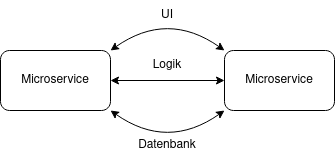
\includegraphics[width=0.60\textwidth]{figures/IntegrationMicroservices.png}
    \caption{Integration von Microservices auf verschiedenen Ebenen \parencite[vgl.][S. 167]{wolffMicroservices2018}}
\end{figure}

Auf Datenbank-Ebene können Microservices integriert werden, indem sie auf dieselbe Datenbank zugreifen. Diese Methode ist einfach zu implementieren, aber bringt einige Nachteile mit sich \parencite[vgl.][S. 69]{newmanMicroservices2015}. Wenn durch Änderungen in einem Microservice die Datenstruktur angepasst wird, wirkt sich das auf die anderen Microservices aus und die Unabhängigkeit wird reduziert. Auch die Technologiefreiheit wird beschränkt. Eigene Datenbanken oder zumindest Datenbankschemata erlauben also mehr Freiheiten und eine schnellere Änderung von Datenstrukturen.

Die Benutzerschnittstelle oder das \ac{UI} ist die Ebene auf der alle Funktionalitäten der Microservices zusammengeführt werden. Um auch hier ein hohe Unabhängigkeit zu gewährleisten, ist es ratsam jeden Microservice mit einer eigenen \ac{UI} auszustatten. Somit können alle Änderungen, egal ob sie \ac{UI}, Logik, oder Datenbank betreffen, von einem Entwicklerteam umgesetzt werden. Das Problem ist jedoch, dass \acp{UI} schnell sehr umfangreich werden und so einen Microservice unnötig groß machen. Außerdem benötigen moderne Anwendungen häufig unterschiedliche Frontends für verschiedene Gerätetypen. Deshalb werden Frontends häufig weiterhin monolithisch aufgebaut. Mittlerweile gibt es jedoch auch immer mehr Micro-Frontends, welche den Microservice-Ansatz auf Frontends übertragen \parencite[vgl.][S. 1]{peltonenMotivations2021}.

Microservices können auch auf Logik-Ebene miteinander verbunden werden. Microservices müssen untereinander kommunizieren, wenn sie die Funktionalität eines anderen Microservices benötigen. Wichtig dabei ist, dass die Microservices trotzdem eine größtmögliche Unabhängigkeit bewahren. Zu viel Kommunikation zwischen zwei Microservices sind ein Hinweis auf eine schlechte Aufteilung \parencite[vgl.][S. 104]{wolffMicroservices2018}. Zyklische Abhängigkeiten sollten unter allen Umständen vermieden werden. Die Kommunikation läuft über \acp{API}. Ein beliebter Architekturstil für \acp{API} ist \ac{REST}. \ac{REST} vereinheitlicht die Struktur und das Verhalten von Schnittstellen \parencite[vgl.][S. 76]{fieldingArchitectural2000}. Bei einer \ac{REST}-\ac{API} gibt es eine Vielzahl von Ressourcen, die über eindeutige \acp{URI}, identifiziert werden. Die Ressourcen können über \acs{HTTP}-Anfragen mit verschiedenen \acs{HTTP}-Anfragemethoden manipuliert werden.

\subsection{Docker}

Anwendungen mit Microservice-Architektur verwenden häufig Containervirtualisierung zur Bereitstellung. Durch die leichtgewichtige Containervirtualisierung können mehrere isolierte Instanzen eines Betriebssystems auf demselben Kernel ausgeführt werden. Dadurch sind die Container ressourcenschonender als die herkömmliche Virtualisierung mittels Hypervisor, bei dem jede virtuelle Maschine ein vollständiges Betriebssystem ausführt \parencite[vgl.][S. 166f]{newmanMicroservices2015}.

\begin{figure}[H] 
    \centering
    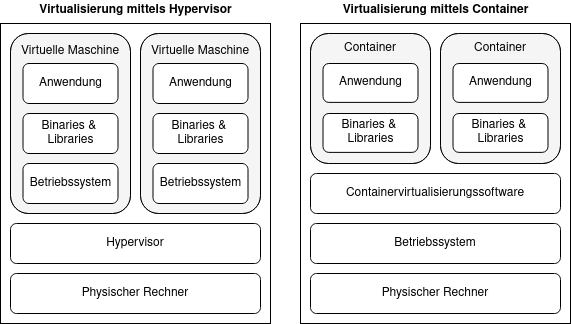
\includegraphics[width=0.95\textwidth]{figures/VergleichVirtualisierung.png}
    \caption{Vergleich Virtualisierung mittels Hypervisor und Container}
\end{figure}

Für die Ausführung einer Anwendung werden Abhängigkeiten wie zum Beispiel Bibliotheken, Compiler und Interpreter benötigt. Des Weiteren muss die Anwendung richtig konfiguriert werden. Vor allem bei einer Microservice-Architektur kann das ein Problem werden, da die Microservices über große Netzwerke verteilt auf verschiedenartigen Rechnern bereitgestellt werden sollen. Containervirtualisierung löst dieses Problem mit einer standardisierten Image-Datei, welche die Anwendung mitsamt aller Abhängigkeiten und Konfigurationen beinhaltet \parencite[vgl.][S. 9]{arundelCloud2019}. Diese Image-Datei läuft unabhängig von der Plattform auf jedem Rechner, sofern die zugehörige Containervirtualisierungssoftware installiert ist.

Eine freie Software zur Containervirtualisierung ist Docker \parencite[vgl.][]{dockerinc.Docker2022}. Sie ist die beliebteste und verbreitetste Software für diesen Zweck und ergänzt die Containervirtualisierung um benutzerfreundliche Werkzeuge \parencite[vgl.][S. 20]{hightowerKubernetes2018}. Docker basiert auf der Virtualisierung mit Linux-Containern. Durch herkömmliche Virtualisierung kann Docker jedoch auch auf anderen Betriebssystemen betrieben werden. Im Folgenden werden die wichtigsten Begriffe und Funktionen von Docker näher beschrieben.

\subsubsection{Docker Image}

Ein Docker Image ist das Speicherabbild eines Containers. Das Image beinhaltet alle Informationen, die zum Starten eines Containers notwendig sind. Bei Docker besteht das Image aus mehreren Schichten. Jede Schicht repräsentiert eine Abhängigkeit oder Konfiguration, welche für die Anwendung benötigt wird. Docker optimiert automatisch den verwendeten Speicherplatz durch Wiederverwendung, wenn zwei Images eine gleiche Schicht benutzen. Die Docker Images sind portabel. Über zentrale Registrys können die Images verwaltet, gespeichert und verteilt werden. DockerHub ist die größte öffentliche Registry mit einer Vielzahl an Images, die von anderen Benutzern bereitgestellt werden. Beim Ausführen eines Images wird auf Basis des Images ein Container gestartet. Das Image ist wiederverwendbar und es können beliebig viele Container aus einem Image erzeugt werden. 

\subsubsection{Dockerfile}

Ein Dockerfile ist eine Textdatei mit mehreren Befehlen, die ein Docker Image beschreiben. Aus einem Dockerfile kann das entsprechende Image gebaut werden. Dazu werden die einzelnen Befehle abgearbeitet und für jeden Befehl eine neue Schicht in dem zugehörigen Image angelegt. Begonnen wird meistens mit einem Basis-Image, welches bereits vorhanden ist. Danach folgen spezifische Änderungen, damit die gewünschte Anwendung ausgeführt werden kann.

\subsubsection{Container}
Ein Container ist die aktive Instanz eines Images. Er besitzt eine begrenzte Lebensdauer und wird nachdem der in ihm laufende Prozess abgeschlossen ist beendet. Container sind in der Regel unveränderlich. Soll ein Container geändert werden, so wird der alte Container gegen einen neuen ausgetauscht. Jeder Container besitzt sein eigenes Dateisystem, Anteil an CPU, Speicher und Prozessraum. Er besitzt auch seine eigenen Bibliotheken, Compiler und Interpreter und ist so unabhängig von allen Softwareversionen, die auf dem eigentlichen Betriebssystem installiert sind. Lediglich der Kernel wird geteilt und bildet die einzige Abhängigkeit. 

\begin{figure}[H] 
    \centering
    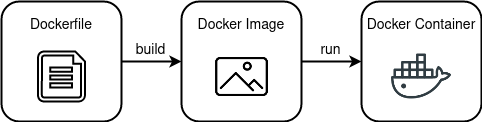
\includegraphics[width=0.8\textwidth]{figures/DockerFileImageContainer.png}
    \caption{Weg vom Dockerfile zum Container}
\end{figure}

\subsection{Kubernetes}

Wenn Microservices in Containern bereitgestellt werden, wird es schnell nicht mehr möglich, die Container manuell zu verwalten. Service Discovery, Skalierung und die Lastverteilung gestalten sich als aufwendige Probleme. Die Open-Source-Plattform Kubernetes versucht diese Probleme zu lösen \parencite[vgl.][]{linuxfoundationKubernetes2022}. Der Name \glqq Kubernetes\grqq{} stammt aus dem griechischen und bedeutet soviel wie Steuermann. Kubernetes hilft bei der Koordination und Sequenzierung verschiedener Aktivitäten sowie bei der Verwaltung der verfügbaren Ressourcen und bei einer effizienten Lastverteilung \parencite[vgl.][S. 11]{arundelCloud2019}. Kubernetes bietet somit viele Funktionen, die die Bereitstellung von Microservices erleichtern. Häufig wird Kubernetes mit Docker verwendet, es unterstützt aber auch andere Anwendungen zur Containervirtualisierung.

\subsubsection{Aufbau}

Die größte Organisationseinheit der Plattform ist ein Kubernetes Cluster. Ein Cluster besteht aus mindestens einem Control Plane und einem Node. Der Control Plane verwaltet sämtliche Nodes. Um Ausfallsicherheit zu gewährleisten können auch mehrere Control Planes in einem Cluster betrieben werden. Ein Control Plane enthählt eine Key-Value-Datenbank namens etcd. In ihr wird die gesamte Konfiguration des Clusters gespeichert. Des Weiteren enthält der Control Plane einen \ac{API}-Server, mit der die Nodes kommunizieren. Auch externe Komponenten können mit dem \ac{API}-Server kommunizieren und so Informationen abfragen, oder das Cluster konfigurieren. Der Controller Manager steuert über den \ac{API}-Server die einzelnen Nodes. Des Weiteren besitzt der Control Plane einen Scheduler, der die Last verteilt und überwacht.

In der Regel besteht ein Cluster aus vielen Nodes. Dabei kann es sich um physische Rechner aber auch um virtuelle Maschinen handeln. Auf den Nodes laufen die Container mit den eigentlichen Anwendungen. Außerdem besitzt jeder Node einen Kubelet. Dieser Kubelet kommuniziert mit dem Controller Manager und verwaltet den Status der Container auf dem jeweiligen Node.

\begin{figure}[H] 
    \centering
    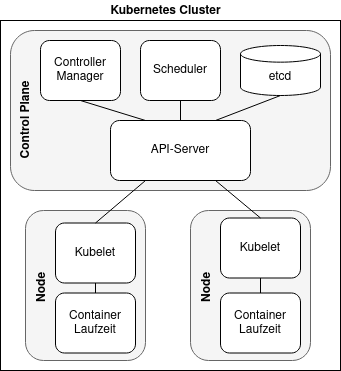
\includegraphics[width=0.60\textwidth]{figures/KubernetesCluster.png}
    \caption{Aufbau eines Kubernetes Clusters}
\end{figure}

\subsubsection{Objekte}

Kubernetes stellt eine Reihe von abstrakten Objekten zur Verfügung, mit denen der Status des Systems dargestellt wird und welche es erleichtern eine Microservice-Architektur zu bauen \parencite[vgl.][S. 13]{hightowerKubernetes2018}. Diese Objekte werden in Manifesten beschrieben. Bei den Manifesten handelt es sich üblicherweise um YAML-Dateien. Die Manifeste sind deklarativ aufgebaut, das bedeutet der gewünschte Ausgangszustand wird beschrieben. Nachdem das Manifest übergeben wurde, führt Kubernetes die entsprechenden Aktionen aus, um den beschriebenen Zustand zu erreichen.

Zu den grundlegenden Objekten gehören die Folgenden:
\begin{itemize}
\item Pods sind die kleinste einsetzbare Einheit. Ein Pod repräsentiert einen einzelnen Container oder eine Gruppe von Containern. Alle Container in einem Pod laufen immer auf dem gleichen Node.
\item Namespaces werden zur logischen Unterteilung des Clusters verwendet. Sie können zur Isolation verschiedener Entwicklerteams oder Anwendungsmodule genutzt werden.
\item Volumes bieten persistenten Speicher, der auch nach der Lebenszeit eines Pods bestehen bleibt.
\item ConfigMaps ermöglichen das Speichern von Konfigurationsdaten als Key-Value-Paare.
\item Labels können anderen Objekten zugeordnet werden, um diese zu Gruppieren.
\item ReplicaSets sorgen dafür, dass eine bestimmte Anzahl von Kopien eines Pods gleichzeitig laufen.
\item Deployments repräsentieren eine zustandslose Anwendung. Deployments verwenden ReplicaSets. Ein Deployment überwacht fortlaufend den Status der Container und kann sie beispielsweise bei Bedarf neu starten.
\end{itemize}

\begin{figure}[H] 
    \centering
    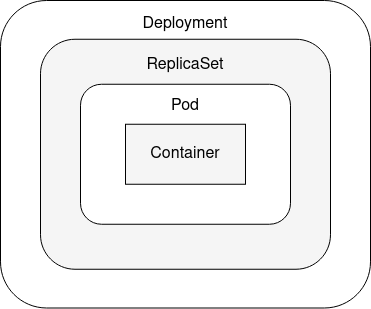
\includegraphics[width=0.55\textwidth]{figures/KubernetesDeployment.png}
    \caption{Aufbau von einem Deployment}
\end{figure}

In den nächsten beiden Abschnitten werden noch weitere Objekte beschrieben, welche für die Service Discovery und die Skalierung nützlich sind.

\subsubsection{Service Discovery}
Kubernetes ist ein dynamisches System. Ein Microservice, der in einem Pod läuft, kann schnell gestoppt, gestartet oder repliziert werden. Da auch mehrere Instanzen eines Microservices gleichzeitig laufen können, wird ein fester Endpunkt benötigt, über den gleichartige Pods erreichbar sind. In Kubernetes kann dafür ein Service-Objekt erstellt werden. Ein Service stellt eine unveränderliche virtuelle IP-Adresse bereit, welche Kubernetes per Lastverteilung auf die passenden Pods verteilt. Innerhalb des Clusters kann ein Service auch über den Service-Namen aufgerufen werden, welcher mit dem \ac{DNS} aufgelöst wird. Ein Service vom Typ ClusterIP ist von außerhalb des Clusters nicht aufrufbar. Mit dem Typ NodePort kann der Service von außen zugänglich gemacht werden. Dazu wird ein fester Port auf allen Nodes geöffnet und der Datenverkehr über diesen Port an den entsprechenden Service weitergeleitet.

\begin{figure}[H] 
    \centering
    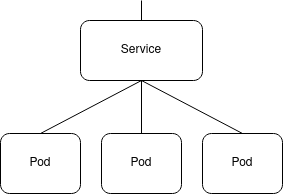
\includegraphics[width=0.55\textwidth]{figures/KubernetesService.png}
    \caption{Service als Endpunkt für mehrere Pods \parencite[vgl.][S. 67]{arundelCloud2019}}
\end{figure}

\subsubsection{Skalierung}

Über ReplicaSets lässt sich eine feste Anzahl von Kopien eines Pods festlegen. In der Praxis soll die Anzahl häufig nach der Auslastung skaliert werden. Diese Aufgabe kann Kubernetes automatisieren. Dafür wird das das Objekt \ac{HPA} angeboten. Mit dem \ac{HPA} kann beispielsweise eine Skalierung in Abhängigkeit der CPU-Auslastung vorgenommen werden. In dem Objekt wird auch angegeben, wie viele Kopien mindestens vorhanden sein sollten und wie viele maximal erstellt werden dürfen. 

\subsubsection{Kubectl}

Kubectl ist der offizielle Kubernetes-Client und dient der Steuerung von Kubernetes. Bei Kubectl handelt es sich um ein \ac{CLI} für die Interaktion mit dem \ac{API}-Server des Control Planes. Mit Kubectl können beispielsweise Objekte verwaltet werden und der Status des gesamten Clusters untersucht werden.

\subsubsection{Minikube}

Minikube ist ein Werkzeug, um ein lokales Kubernetes Cluster zu betreiben. Minikube erstellt ein Cluster bestehend aus nur einem Node in einer virtuellen Maschine. Der Node fungiert dabei sowohl als Control Plane sowie auch als Node. Minikube unterstützt mittlerweile auch den Betrieb mit mehreren Nodes. Des Weiteren kann das gesamte Cluster selbst auch in einem Docker Container anstatt in einer virtuellen Maschine betrieben werden. Minikube erstellt beim Start automatisch eine Kubectl-Konfiguration, welche auf das Cluster zeigt. Dadurch kann das Cluster mithilfe von Kubectl gesteuert werden. 